\documentclass[10pt]{article}

\usepackage{spheric}
%%%TITLE
\title{High speed water impacts of flat plates in different ditching configurations through a Riemann-ALE SPH model}
\date{}

%%AFFILIATIONS
\author[1]{S. Marrone}
\author[1,3]{A. Colagrossi}
\author[2]{M. De Leffe}
\author[2]{L. Chiron}
\author[3]{D. Le Touz\'e}

\affil[1]{CNR-INSEAN, - Marine Tech. Research Inst., Rome, Italy}
\affil[2]{NEXTFLOW Software, Nantes, France} 
\affil[3]{\'Ecole Centrale Nantes, LHEEA research dept., Nantes, France}

%%DOCUMENT
\begin{document}

\maketitle

%%PLEASE PUT YOUR ABSTRACT HERE
\begin{abstract}
The violent water entry of flat plates is investigated through a Riemann-ALE SPH model. The test conditions are of interest for problems related to aircraft and helicopter emergency landing in water. Three main parameters are considered: the horizontal velocity, the approach angle (i.e. vertical to horizontal velocity ratio) and the pitch angle, $\alpha$. Regarding the latter, small angles are considered in this study. As described in the theoretical work by Zhao and Faltinsen (1993), for small $\alpha$ a very thin, high-speed jet of water is formed, and the time-spatial gradients of the pressure field are extremely high. Further, air-entrainment can take place making even more complex the loading process of the plate. These test conditions are very challenging for numerical solvers. In the present study an enhanced SPH model \cite{oger2016sph} is firstly tested on a purely vertical impact with deadrise angle $\alpha=4^\circ$ (Fig. \ref{fig:1-1}). An in-depth validation against analytical solutions and experimental results is carried out, highlighting the several critical aspects of the numerical modelling of this kind of flow, especially when pressure peaks are to be captured (left plot of Fig. \ref{fig:1-2}). A discussion on the main difficulties when comparing to model scale experiments is also provided. Then, the more realistic case of a plate with both horizontal and vertical velocity components is discussed and compared to ditching experiments recently carried out at CNR-INSEAN \cite{iafrati2016experimental}. In this case both single and two-phase models are considered to take into account possible air-cushion effects (right plot of Fig. \ref{fig:1-2}).
\begin{figure}[!htb]
\centering
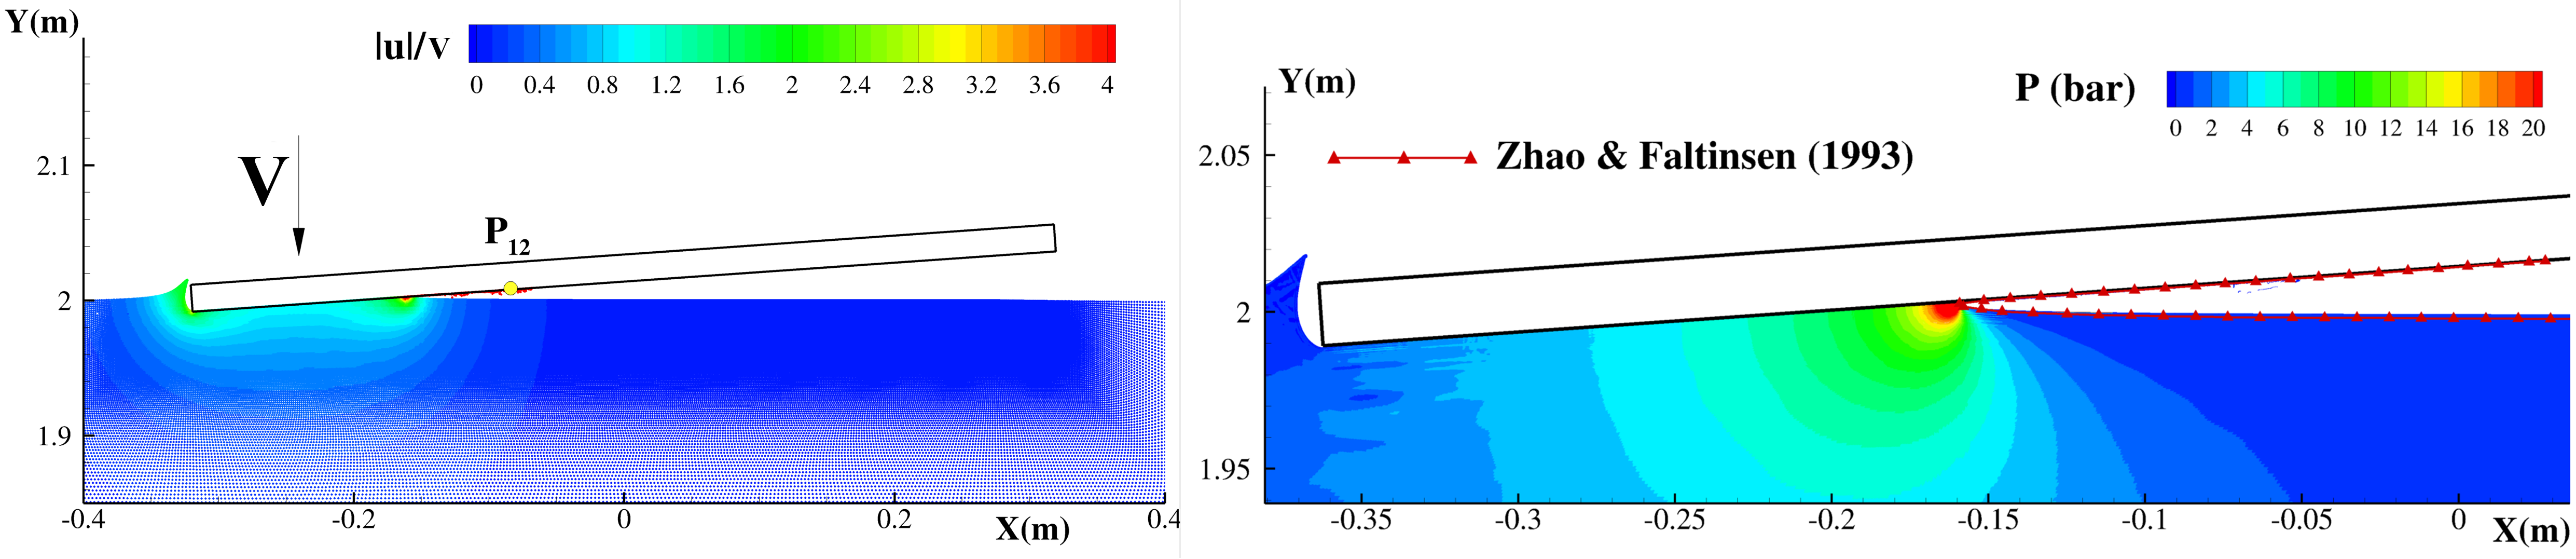
\includegraphics[width=0.9\textwidth]{1-1.png}
\caption{Water entry of a plate at $U = 0$, $V = -6~\mathrm{m/s}$ with $4^\circ$ pitch angle. Left: contour plot of the flow velocity magnitude. Right: contour plot of the pressure field.}\label{fig:1-1}
\end{figure}
\begin{figure}[!htb]
\centering
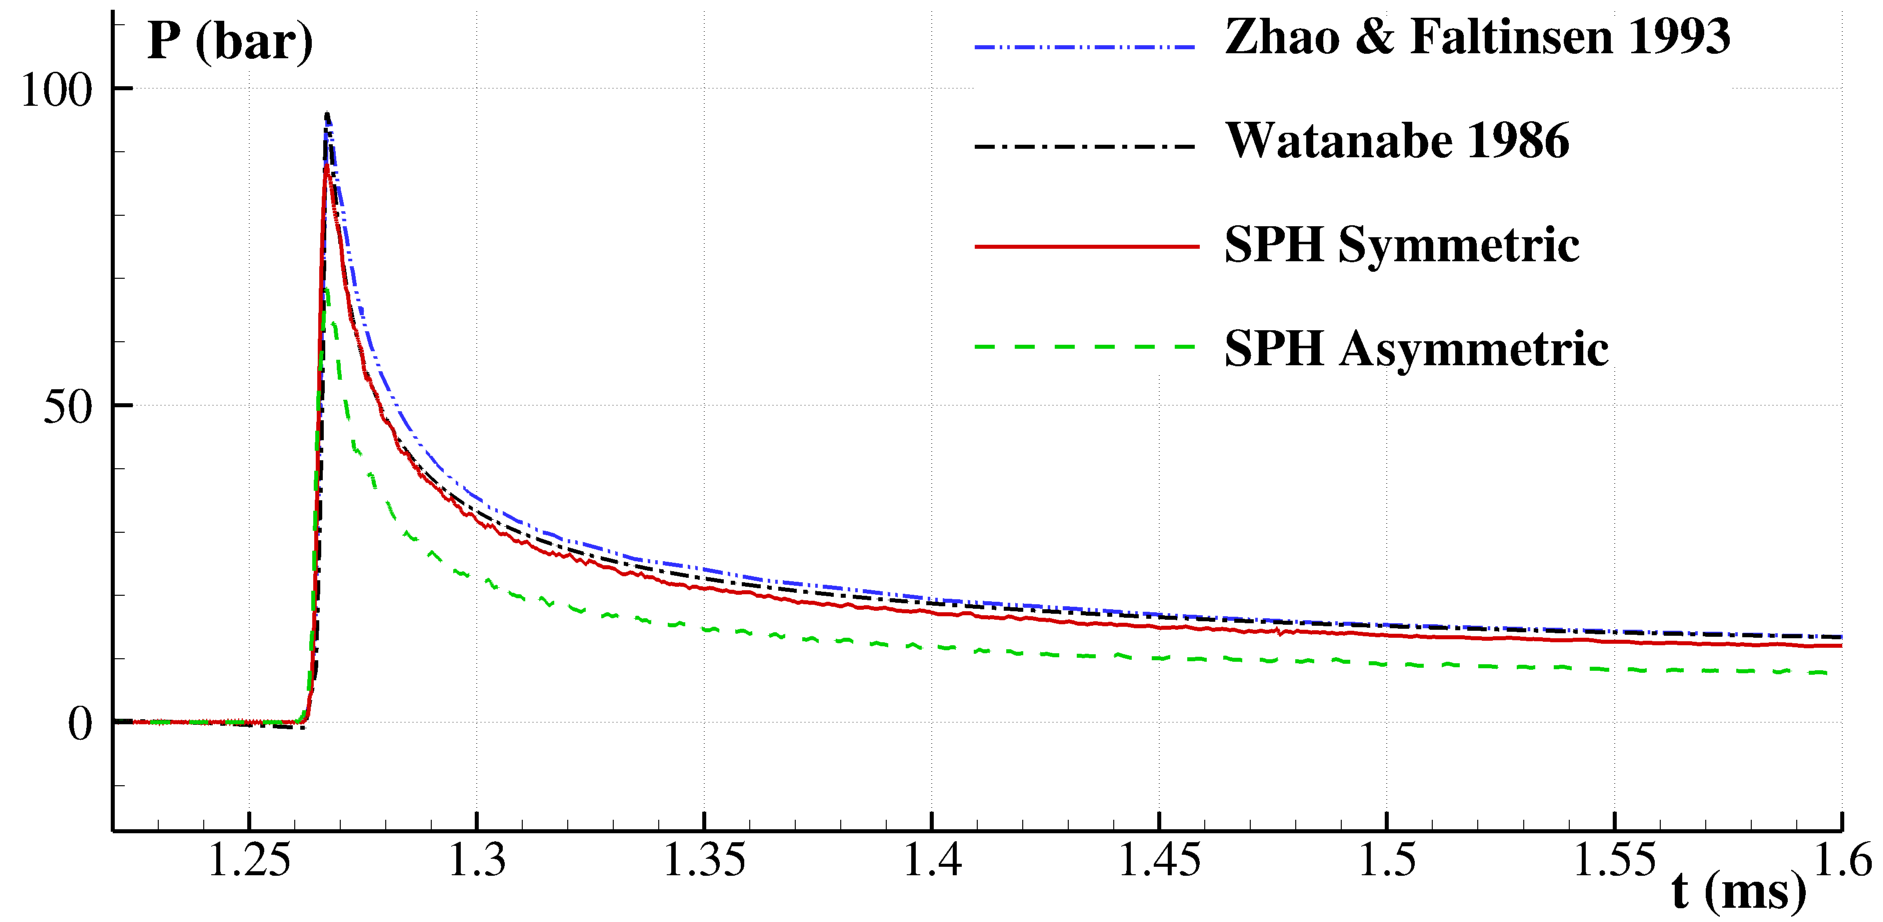
\includegraphics[width=0.45\textwidth]{1-21.png}~~~~~
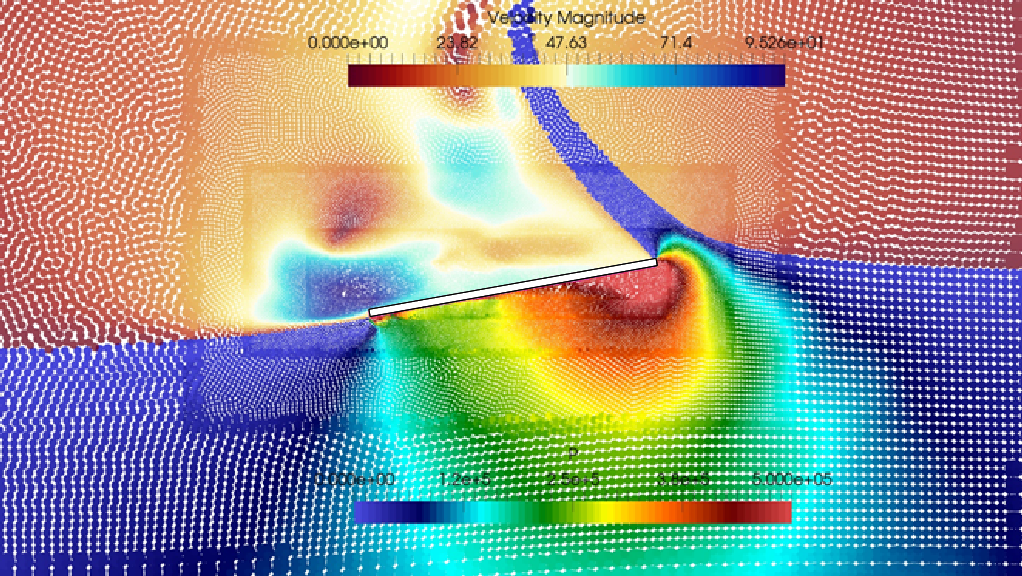
\includegraphics[width=0.385\textwidth]{1-22.png}
\caption{Left: pressure measured at probe $P_{12}$ (see Fig. 1) with SPH in asymmetric and symmetric configurations and comparison with analytical solutions. Right: Two-phase water entry of a plate at $U = 40$, V$ = -1.5~\mathrm{m/s}$ with $10^\circ$ pitch angle.}\label{fig:1-2}
\end{figure}
\end{abstract}

\addbib
\end{document}
